%15 min preso!
\documentclass[xcolor=table,aspectratio=169]{beamer}
\usepackage{beamerthemesplit}
\usepackage{wrapfig}
\usetheme{SPbGU}
\usepackage{pdfpages}
\usepackage{amsmath}
\usepackage{cmap}
\usepackage[T2A]{fontenc}
\usepackage[utf8]{inputenc}
\usepackage[english]{babel}
\usepackage{indentfirst}
\usepackage{amsmath}
\usepackage{tikz}
\usepackage{multirow}
\usepackage[noend]{algpseudocode}
\usepackage{algorithm}
\usepackage{algorithmicx}
\usepackage{fancyvrb}
\usepackage{hyperref} 
\usetikzlibrary{calc}
\usetikzlibrary{shapes}
\usetikzlibrary{arrows,automata}
\usetikzlibrary{positioning}
\usetikzlibrary{fit}
\usetikzlibrary{shapes.callouts}
\usetikzlibrary{shapes.misc}
\usepackage{xparse}

\usepackage{etoolbox,refcount}
\usepackage{multicol}

\usepackage{fontawesome5}
\usepackage{fontawesome}

\usepackage{tabularx}
\newcolumntype{Y}{>{\raggedleft\arraybackslash}X}

\renewcommand{\thealgorithm}{}

\newtheorem{mytheorem}{Theorem}
\renewcommand{\thealgorithm}{}

\newcommand{\tikzmark}[1]{\tikz[overlay,remember picture] \node (#1) {};}
\def\Put(#1,#2)#3{\leavevmode\makebox(0,0){\put(#1,#2){#3}}}

\newcommand{\ltz}{$< 1$}

\tikzset{
    state/.style={
           rectangle,
           rounded corners,
           draw=black, very thick,
           minimum height=2em,
           inner sep=2pt,
           text centered,
           },
}

\tikzset{
    invisible/.style={opacity=0,text opacity=0},
    visible on/.style={alt=#1{}{invisible}},
    alt/.code args={<#1>#2#3}{%
      \alt<#1>{\pgfkeysalso{#2}}{\pgfkeysalso{#3}} % \pgfkeysalso doesn't change the path
    },
}

\tikzset{cross/.style={cross out, draw=black, minimum size=2*(#1-\pgflinewidth), inner sep=0pt, outer sep=0pt, ultra thick},
%default radius will be 1pt. 
cross/.default={1pt}}

\NewDocumentCommand{\mycallout}{r<> O{opacity=0.8,text opacity=1} m m m}{%
\tikz[remember picture, overlay]\node[align=center, fill=cyan!20, text width=#5cm,
#2,visible on=<#1>, rounded corners,
draw,rectangle callout,anchor=pointer,callout relative pointer={(290:0.5cm)}]
at (#3) {#4};
}

\NewDocumentCommand{\mycalloutR}{r<> O{opacity=0.8,text opacity=1} m m m}{%
\tikz[remember picture, overlay]\node[align=center, fill=cyan!20, text width=#5cm,
#2,visible on=<#1>, rounded corners,
draw,rectangle callout,anchor=pointer,callout relative pointer={(30:0.8cm)}]
at (#3) {#4};
}


%callout relative pointer={(230:0.5cm)}]

\newcounter{countitems}
\newcounter{nextitemizecount}
\newcommand{\setupcountitems}{%
  \stepcounter{nextitemizecount}%
  \setcounter{countitems}{0}%
  \preto\item{\stepcounter{countitems}}%
}
\makeatletter
\newcommand{\computecountitems}{%
  \edef\@currentlabel{\number\c@countitems}%
  \label{countitems@\number\numexpr\value{nextitemizecount}-1\relax}%
}
\newcommand{\nextitemizecount}{%
  \getrefnumber{countitems@\number\c@nextitemizecount}%
}
\newcommand{\previtemizecount}{%
  \getrefnumber{countitems@\number\numexpr\value{nextitemizecount}-1\relax}%
}
\makeatother    
\newenvironment{AutoMultiColItemize}{%
\ifnumcomp{\nextitemizecount}{>}{3}{\begin{multicols}{2}}{}%
\setupcountitems\begin{itemize}}%
{\end{itemize}%
\unskip\computecountitems\ifnumcomp{\previtemizecount}{>}{3}{\end{multicols}}{}}


\beamertemplatenavigationsymbolsempty

\title[All You Need is Generalized GLL]{All You Need is Generalized GLL}
\subtitle{Parsing algorithms are not only about string processing}
%\institute[PL\&T@SPbSU]{
%Saint Petersburg State University
%}

% То, что в квадратных скобках, отображается в левом нижнем углу.
\author[Semyon Grigorev]{Semyon Grigorev}

\date{December 29, 2022}

\begin{document}
{
\begin{frame}[fragile]
  \begin{table}
  \centering
  \begin{tabularx}{\linewidth}{XcX}
    
\includegraphics[height=0.9cm]{pictures/hu_logo.jpeg} \hfill
    & 
    & \hfill 
\includegraphics[height=1.6cm]{pictures/SPbGU_Logo.png}
  \end{tabularx}
  \end{table}
  \titlepage
\end{frame}
}



\begin{frame}[fragile]
  \frametitle{Generalized Parsing}  
  \tikzset{dbl/.style={double,double distance=2pt}} 
  \begin{minipage}[t]{0.49\textwidth}
    \begin{itemize}
      \item Handles arbitrary context-free grammars
      \begin{itemize}
        \item Ambiguous
        \item (Hidden) Left-recursive (for LL)
      \end{itemize}
      \item Linear for unambiguous grammars 
      \item Cubic in worst case
    \end{itemize}
  \end{minipage}
  \pause  
  \begin{minipage}[t]{0.49\textwidth}
    \begin{itemize}
      \item ANTLR: ALL(*)
      \item Tree-Sitter: GLR
      \item SDF3 (Spoofax): GLR
      \item \ldots
    \end{itemize}
  \end{minipage}
  \vfill
  \pause
  \begin{itemize}
    \item GSS --- Graph Structured Stack, compact representation of stack
    \item SPPF --- Shared Packed Parse Forest, compact representation of parse forest
  \end{itemize}
\end{frame}

\begin{frame}[fragile]
  \frametitle{Generalized LL (GLL)\footnote{\href{https://www.cwi.nl/nieuws/2019/thesis_final-1.pdf}{A. Afroozeh, A. Izmaylova. ``Practical General Top-Down Parsers''. 2019.}}}  
  \begin{minipage}[t]{0.48\textwidth}
  \begin{itemize}
    \item Descriptor
    \begin{itemize}
      \item Grammar slot: $S \to a \cdot S b$
      \item Input position
      \item Top element of stack
      \item Root of tree
    \end{itemize}   
  \end{itemize}
\end{minipage}
\pause
\begin{minipage}[t]{0.48\textwidth}
  \begin{itemize}
    \item Step --- handle one descriptor
    \item Step produces a \underline{\textbf{set}} of new descriptors
    \item Each descriptor handle once 
    \begin{itemize}
      \item Set of handled descriptors
      \item Order does not matter
    \end{itemize}
  \end{itemize}   
\end{minipage}
\pause
\vfill
\begin{itemize}
  \item \href{https://github.com/iguana-parser/iguana}{Iguana} --- GLL-based parser generator
\end{itemize}
\end{frame}

\begin{frame}[fragile]
  \frametitle{EBNF Without Transformation}
  \begin{center}
    \begin{tabular}{l | r}
      $S \to \varepsilon \mid S a$\hspace{3cm} & \hspace{3cm} $S \to a^*$ \\
      \pause
      & \\
      $S \to \varepsilon \mid a S b S \mid c S d S$ & $S \to (a S b \mid c S d) ^ *$ \\
    \end{tabular}
  \end{center}
  \vfill
  \pause
  \begin{itemize}
    \item Slot --- state of DFA (right part of rule)
    \pause
    \item Careful handling of descriptor
    \begin{itemize}
      \item Both terminal and nonterminal can be the next symbols for the current state at the same time
      \item Multiple different nonterminals can be the next symbols for the current state
      \item State can be final and contains outgoing edges
    \end{itemize}
    \pause
    \item SPPF becomes more complex     
  \end{itemize} 
\end{frame}

\begin{frame}[fragile]
  \frametitle{Nonlinear Input Handling}
  \vspace{-0.5cm}
  \begin{center} String = linear graph \\
  \begin{tikzpicture}[shorten >=1pt,node distance=1.5cm,on grid,auto]
  \tikzstyle{point} = [circle, minimum width = 3pt, fill]
     \node[point] (a) {};
     \node[point] (b)[right=of a] {};
     \node[point] (c)[right=of b] {};
     \node[point] (d)[right=of c] {};
     \node[point] (e)[right=of d] {};
     \node[point] (f)[right=of e] {};
     \node[point] (g)[right=of f] {};
     \path[->]
      (a) edge node {S} (b)
      (b) edge node {T} (c)
      (c) edge node {R} (d)
      (d) edge node {I} (e)
      (e) edge node {N} (f)
      (f) edge node {G} (g);
  \end{tikzpicture}
  \end{center}
  
  \bigskip 
  
  %\bigskip 
  
  \pause
  
  \begin{center} What makes a graph \textbf{not} a string? \end{center}
  
  \pause 
  
  \begin{multicols}{2}
  \begin{center} Branches \end{center}
  
  \begin{multicols}{2}
  \begin{center}
  \begin{tikzpicture}[shorten >=1pt,node distance=1.4cm,on grid,auto]
  \tikzstyle{point} = [circle, minimum width = 2.5pt, fill]
     \node[point] (a) {};
     \node[point] (b)[right=of a, above right=of a] {};
     \node[point] (c)[right=of a, below=of b] {};
     \path[->]
      (a) edge node {A} (b)
      (a) edge[below] node {B} (c);
  \end{tikzpicture}
  \end{center}
  
  \columnbreak
  
  \begin{center}
  \begin{tikzpicture}[shorten >=1pt,node distance=1.4cm,on grid,auto]
  \tikzstyle{point} = [circle, minimum width = 2.5pt, fill]
     \node[point] (a) {};
     \node[point] (b)[left=of a, above left=of a] {};
     \node[point] (c)[left=of a, below=of b] {};
     \path[->]
      (b) edge node {A} (a)
      (c) edge[below] node {B} (a);
  \end{tikzpicture}
  \end{center}
  \end{multicols}
  
  \columnbreak 
  
  \pause
  
  \begin{center} Cycles \end{center}
  \begin{center}
  \begin{tikzpicture}[shorten >=1pt,node distance=1.4cm,on grid,auto]
  \tikzstyle{point} = [circle, minimum width = 2.5pt, fill]
     \node[point] (a) {};
     \node[point] (b)[right=of a] {};
     \node[point] (c)[below=of b] {};
     \node[point] (d)[left=of c] {};
     \path[->]
      (a) edge node {Y} (b)
      (b) edge node {A} (c)
      (c) edge node {D} (d)
      (d) edge node {A} (a);
  \end{tikzpicture}
  \end{center}
  \end{multicols}
  \pause
  \vspace{-0.6cm}
  \begin{itemize}
    \item Multiple different terminals can be the next symbols for the current state
    \item Each descriptor handle once (cycles and merges not a problem)
  \end{itemize}
  \end{frame}


\begin{frame}[fragile]
  \frametitle{Error Recovery}
  \begin{itemize}
    \item Language Editing Distance (LED): for the given language $\mathcal{L}$ and the given string $w$ to find string $w_1$ such that $w_1 \in \mathcal{L}$, \texttt{dist}$(w,w_1)$ is minimal 
  \end{itemize}
  \pause
  \begin{center}
  \begin{tikzpicture}[shorten >=1pt,node distance=2.3cm,on grid,auto]
    \tikzstyle{point} = [circle, minimum width = 3pt, fill]
       \node[point] (a) {};
       \node[point] (b)[right=of a] {};
       \node[point] (c)[right=of b] {};
       \node[point] (d)[right=of c] {};
       \node[point] (e)[right=of d] {};
       \node[point] (f)[right=of e] {};
       \node[point] (g)[right=of f] {};
       \path[->]
        (a) edge node {S,0} (b)
        (b) edge node {T,0} (c)
        (c) edge node {R,0} (d)
        (d) edge node {I,0} (e)
        (e) edge node {N,0} (f)
        (f) edge node {G,0} (g)
        (a) edge [bend left=50,draw=none] node [draw=none] {\phantom{$r_1,1$}} (b)
        (a) edge [loop below, draw=none] node [draw=none] {\phantom{$i_1,1$}} (a)
        (g) edge [loop below, draw=none] node [draw=none] {\phantom{$i_1,1$}} (g)
        (a) edge [bend right=40,draw=none] node [draw=none] { } (b);
      \path<3->[->]
      (a) edge [bend right=40] node {$\varepsilon,1$} (b);
      \path<4->[->]
      (a) edge [bend left=50] node {$r_1,2$} (b);
      \path<5->[->]
      (a) edge [loop below] node {$i_1,1$} (a);
      \path<6->[->]
      (b) edge [bend right=40] node {$\varepsilon,1$} (c)
      (b) edge [bend left=50] node {$r_2,2$} (c)
      (b) edge [loop below] node {$i_2,1$} (b);
      \path<7->[->]
      (c) edge [bend right=40] node {$\varepsilon,1$} (d)
      (c) edge [bend left=50] node {$r_3,2$} (d)
      (c) edge [loop below] node {$i_3,1$} (c);
      \path<8->[->]
      (d) edge [bend right=40] node {$\varepsilon,1$} (e)
      (d) edge [bend left=50] node {$r_4,2$} (e)
      (d) edge [loop below] node {$i_4,1$} (d);
      \path<9->[->]
      (e) edge [bend right=40] node {$\varepsilon,1$} (f)
      (e) edge [bend left=50] node {$r_5,2$} (f)
      (e) edge [loop below] node {$i_5,1$} (e);
      \path<10->[->]
      (f) edge [bend right=40] node {$\varepsilon,1$} (g)
      (f) edge [bend left=50] node {$r_6,2$} (g)
      (f) edge [loop below] node {$i_6,1$} (f);
      \path<11->[->]
      (g) edge [loop below] node {$i_7,1$} (g);
    \end{tikzpicture}  
  \end{center}
  \onslide<12->{
  
  \begin{itemize}
    \item Error recovery $\to$ find a minimal weight path from start to final in the given graph which forms a word in the given language
    \item Set of descriptors to handle $\to$ priority queue
  \end{itemize}
  }
\end{frame}


\begin{frame}[fragile]
  \frametitle{Path Querying}  
  \begin{minipage}[m]{0.45\linewidth}
    \raisebox{-0.5\totalheight}{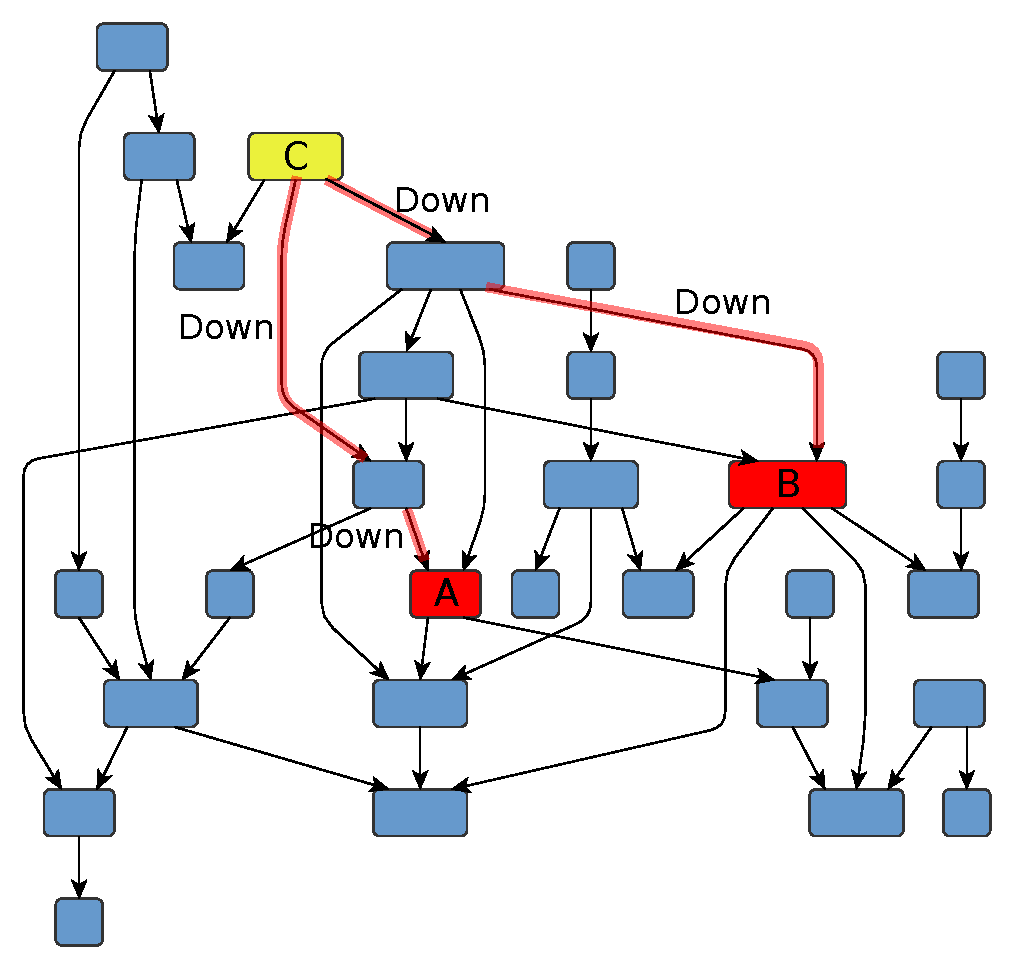
\includegraphics[width=\textwidth]{pictures/hierarchical.pdf}}
    \end{minipage}\hfill
    \begin{minipage}[m]{0.5\linewidth}
    \textbf{Context-free} languages as constraints (CFPQ, Context-Free Path Querying)
    \begin{itemize}
          \item Are nodes A and B on the same level of hierarchy?
          \item Is there a path of form $\overline{\textbf{Down}}^n \, \textbf{Down}^n$ between A and B?
          \item Context-free grammar: $\textit{SameLvl} \to \overline{\textit{Down}} \ \textit{SameLvl} \ \textit{Down} \mid \varepsilon$
    \end{itemize}
    \pause
  
    \vspace{0.3cm}
  
  
    Applications
      \begin{itemize}
        \item Static code analysis [\href{https://dl.acm.org/doi/10.1145/199448.199462}{T. Reps, et al, 1995}]
        \item Graph segmentation [\href{https://dblp.org/rec/conf/icde/0001D19.html}{H. Miao, et al, 2019}]
        \item Biological data analysis [\href{https://pubmed.ncbi.nlm.nih.gov/20134073/}{P. Sevon, et al, 2008}] \ldots
      \end{itemize}
  
    \end{minipage}
  
\end{frame}


\begin{frame}[fragile]
  \frametitle{Conclusion}  
  \begin{itemize}
    \item Generalized parsing opens the door to
    \begin{itemize}
      \item Arbitrary context-free grammars handling
      \item Natural error recovery
      \item Graph navigation
      \item \ldots
    \end{itemize} 
  \end{itemize}
\end{frame}


\end{document}
